Relaciona la imagen con  el tipo de onda electromagnética que está involucrada.
\begin{multicols}{2}
    \begin{flushright}
        \adjustbox{valign=t}{
\includegraphics[width=0.2\textwidth ]{../images/SINFI_U3_AC77_IMG4.png} }
        $\square$\\
        \adjustbox{valign=t}{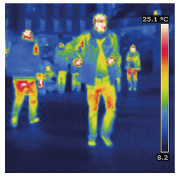
\includegraphics[width=0.2\textwidth ]{../images/SINFI_U3_AC77_IMG5.png} }
        $\square$\\
        \adjustbox{valign=t}{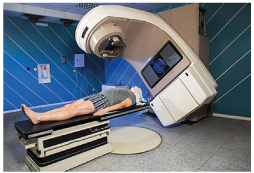
\includegraphics[width=0.2\textwidth ]{../images/SINFI_U3_AC77_IMG6.png} }
        $\square$\\
        \adjustbox{valign=t}{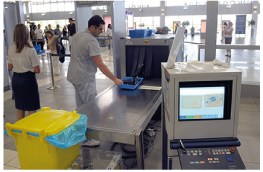
\includegraphics[width=0.2\textwidth ]{../images/SINFI_U3_AC77_IMG7.png} }
        $\square$\\
    \end{flushright}
    \vspace{1cm}
    \begin{checkboxes}
        \choice Rayos X                 \vspace{2cm}
        \choice Rayos gamma             \vspace{2cm}
        \choice Radiación infraroja     \vspace{2cm}
        \choice Rayos ultravioleta      \vspace{2cm}
    \end{checkboxes}
\end{multicols}